\pagestyle{plain}

\newcommand{\subtitulo}[1]{\NoCaseChange{\textnormal{\break\Large\itshape#1}}}
\chapter*{Introdução\smallskip\subtitulo{Um clássico da etnologia\\ sul-americanista}}
\markboth{Introdução}{Peter Schröder}
\addcontentsline{toc}{chapter}{Introdução, \textit{por Peter Schröder}}

%\formular\itshape

\begin{flushright}
\textsc{peter schröder}\medskip
\end{flushright}

\noindent{}\textit{Die Aruaken}, livro raro que apenas pode ser encontrado em poucos sebos, é uma síntese dos conhecimentos sobre os povos indígenas falantes de línguas aruaques\footnote{Também conhecida como \textit{aruak} ou \textit{arawak}.} escrito durante o período da Primeira Guerra Mundial. Um trabalho clássico de suma importância para os estudos comparativos destes povos,\footnote{Como pode ser observado pela leitura de diversos artigos na coletânea organizada por Hill \& Santos"-Granero, de 2002.} é também a segunda tese de doutorado de Max Schmidt.\footnote{O autor já havia doutorado"-se em Direito pela Friedrich"-Alexander"-Universität Erlangen desde 1899, e realizado três expedições científicas na América do Sul, entre 1900--01, 1910 e 1914.}

Depois de voltar da primeira expedição, em 1901, Schmidt obtém emprego, como assistente da diretoria, no Real Museu Etnológico em Berlim --- então, um centro de estudos etnológicos americanistas na Alemanha. Em 1916, ele defende sua segunda tese na Faculdade de Filosofia da Universidade de Leipzig que dá origem, um ano depois, a esta publicação, tradicionalmente obrigatória para a recepção do título de doutor\footnote{\textit{Dr.\,phil.} neste caso, segundo a credencial alemã.} no sistema universitário alemão.

O interesse acerca da expansão territorial dos povos aruaques nas terras baixas da América do Sul deriva de suas observações, durante as expedições, acerca da influência cultural destes povos sobre grupos linguística e culturalmente diferenciados. Segundo o autor, o problema central do estudo não seria descobrir a origem geográfica dos Aruaques, mas explicar sua dinâmica cultural --- o que, na prática, não pôde ser feito sem alguma abordagem do primeiro ponto.\footnote{A forma como tratou esta dinâmica de fato indica caminhos para rumos posteriores da antropologia, enquanto a questão da origem remete a interesses predominantes na etnologia alemã do século \textsc{xix}.} É apenas no quinto capítulo de \textit{Os Aruaques} que Schmidt aventa uma hipótese sobre a possível origem geográfica destes povos no sudoeste da Amazônia, operando com especulações sobre contatos com as culturas do altiplano andino, como \textit{tiwanaku}.

%e na operação com distinções claras entre fenômenos como língua e cultura,
Talvez sua excepcionalidade enquanto pesquisador esteja na proposta de problematização das diferenças entre classificações linguísticas e características culturais, e conceitos como \textit{aculturação}, \textit{difusão} e \textit{mudança cultural} em termos gerais. Seu principal argumento epistemológico é de que outros autores, anteriores a ele, não teriam levantado as questões certas sobre a expansão dos povos aruaques e, por isso, não teriam chegado a respostas satisfatórias. É neste sentido que devemos, portanto, perceber o aspecto original e inovador de sua teoria à época em que foi escrita.

\section{A estrutura e o método}

A estrutura do texto consiste em comentários metodológicos e um resumo dos estudos etnológicos realizados sobre os povos aruaques até então. O autor escreve sobre os motivos, os meios e o caráter\footnote{Seguindo os três temas citados, se encontram respectivamente nos segundo, terceiro e quarto capítulos.} de sua expansão. Desenvolve a teoria, a partir daí, no sentido de tratar da posição destes povos com relação a outras culturas indígenas e não indígenas nas Américas, de examinar a influência de sua expansão sobre as transformações das manifestações culturais.\footnote{Os dois temas podem ser encontrados, respectivamente, nos quinto e sexto capítulos.} 

Nos comentários que precedem o texto principal --- o primeiro capítulo do livro ---,\footnote{Chamado \textit{Methodologische Vorbemerkungen}, em alemão.} o autor explica seu posicionamento teórico e metodológico por meio da \emph{defesa da interdisciplinaridade} e da autodenominada \emph{abordagem sociológica}. Inicialmente, a posição em relação à \textit{doutrina dos círculos culturais}\footnote{\textit{Kulturkreislehre}, em alemão.} de Fritz Graebner e do padre~Wilhelm~Schmidt ainda pode ser descrita como reservada e cautelosa, porém se transforma em uma rejeição contundente ao final do trabalho. 

Do ponto de vista metodológico, Schmidt, com sua defesa de comparações interculturais sistemáticas e empiricamente fundamentadas, se posiciona mais próximo dos ensinamentos de Franz Boas do que das \textit{teorias difusionistas} austro"-alemãs da época, refletindo as influências de Adolf Bastian e Karl von den Steinen.
% \footnote{\textit{Kulturkreislehre}, em alemão.} de Fritz Graebner\footnote{1877--1934.} e do padre~Wilhelm~Schmidt\footnote{1868--1954.} ainda pode ser descrita como reservada e cautelosa, porém se transforma em uma rejeição contundente ao final do trabalho. Do ponto de vista metodológico, Schmidt, com sua defesa de comparações interculturais sistemáticas e empiricamente fundamentadas, se posiciona mais próximo dos ensinamentos de Franz Boas\footnote{1858--1942.} do que das \textit{teorias difusionistas} austro"-alemãs da época, refletindo as influências de Adolf Bastian\footnote{1826--1905.} e Karl von den Steinen.\footnote{1855--1929.}

O caráter do estudo é etnológico, no sentido de uma comparação sistemática de informações etnográficas. Para as análises bibliográficas, Schmidt lançou mão, além dos próprios trabalhos sobre os \textit{paressí"-kabiší},\footnote{Ou \textit{paresí"-kabizi}.} principalmente dos estudos de autores como Paul Ehrenreich, Theodor Koch"-Grünberg, Erland Nordenskiöld, Karl von den Steinen e Everhard im Thurn, este com relação às Guianas. De modo geral, as explicações e digressões etnográficas do autor são basicamente ilustrativas, limitando"-se a dar sustento a sua teoria explicativa sobre a expansão social e cultural dos aruaques.
% Paul Ehrenreich,\footnote{1855--1914.} Theodor Koch"-Grünberg,\footnote{1872--1924.} Erland Nordenskiöld,\footnote{1877--1932.} Karl von den Steinen\footnote{1855--1929.} e Everhard im Thurn,\footnote{1852--1932.} este com relação às Guianas.

\section{A análise da expansão}

A análise parte da identificação da agricultura, tendo no cultivo de milho e mandioca os fatores economicamente dominantes, combinada com uma maior complexidade social, como denominador comum de todas as culturas aruaques, apesar de sua grande diversidade em termos gerais. É curioso, vista a relevância para os estudos atuais de economias indígenas, que as numerosas variedades destas culturas agrícolas ainda não tenham sido levadas em consideração.

Desse modo, a abordagem \textit{sociológica} de Schmidt também poderia ser
rotulada como \textit{socioeconômica},\footnote{Embora não deva ser confundida com um
simples determinismo materialista, vista sua diferença em relação às teorias
predominantes na etnologia alemã da época.} ilustrada pela seguinte cadeia de 
consequências apresentada pelo autor:
%\medskip

\begin{figure}[H]
  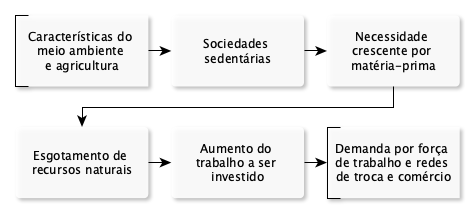
\includegraphics[width=\textwidth]{./TABELA.png}  
\end{figure}

%\medskip
Neste sentido, ele parece antecipar em parte a
ecologia cultural de Julian Steward.
%\footnote{1902--1972.}

As formas de organização social dos Aruaques são analisadas com relação às atividades econômicas e às diferenciações sociais internas. Sua expansão seria menos populacional, no sentido de grupos inteiros se deslocarem para novos territórios, mas, sobretudo, caracterizada por dominação social e cultural. 

A necessidade de manter o sedentarismo nas comunidades desencadearia processos de procura por ampliação da força de trabalho não mais encontrada nas mesmas, porém a incorporação de membros de outras se daria tanto por subjugação militar quanto, majoritariamente, por influências culturais exercidas de forma lenta e sutil, de modo que a expansão dos Aruaques possa ser chamada \textit{sociocultural}. 

Neste sentido, serão analisadas as mais diversas formas, relatadas nas etnografias consultadas, de relações entre Aruaques e não Aruaques: conflitos com outros povos com o objetivo de roubar ou escravizar mulheres e crianças, casamentos por rapto,\footnote{Ou \textit{Raubehe}.} dominação militar, alianças políticas, casamentos interétnicos pacificamente regularizados, adoções, visitas, festas, rituais, trocas de objetos, etc. 

Até o ritual da \textit{couvade} é interpretado neste sentido: no caso de residência pós"-nupcial uxorilocal,\footnote{Costume tradicional no qual os cônjuges casados se mudam para a casa da esposa ou para a sua localidade.} sua função seria socialmente agregativa por conseguir vincular genros à unidade doméstica do sogro (aruaque).

Além desses mecanismos de dominação, Schmidt apresenta uma série de outros que poderiam ser rotulados de \textit{ideológicos}, num sentido quase marxista: mitos, determinados rituais e magias. Até as artes plásticas serão interpretadas como tendo essa função social.

\section{Uma teoria funcionalista e dinâmica}

Sua teoria sobre o caráter e as causas da expansão aruaque nas terras baixas da América do Sul tem pouco a ver com as teorias migratórias da época por identificar e explicitar diversos fatores sociais e econômicos. Foi assim que ele conseguiu apresentar uma teoria própria de mudança cultural, ao mesmo tempo funcionalista e dinâmica, melhor caracterizada como uma teoria de sobreposição social e cultural engatada com algum tipo de teoria de dependência \textit{avant le nom}. 

Os Aruaques transformam em dependentes outros grupos ou povos antes independentes por contribuir à satisfação das necessidades econômicas destes e, ao mesmo tempo, de si mesmos. Nas palavras do autor, ``Correspondem então, por um lado, o instinto de ganho e, por outro lado, o instinto de subjugação''.\footnote{No original alemão: \textit{Es entsprechen sich also der Erwerbstrieb auf der einen Seite und der Unterwerfungstrieb auf der anderen Seite}.} Um vocabulário, ainda que ultrapassado, indicador de uma leitura inovadora.

Schmidt lança uma crítica contundente\footnote{Pode ser encontrada no sexto capítulo.} contra o padre Wilhelm Schmidt e a \textit{doutrina dos círculos culturais}, em particular contra sua aplicação para explicar a diversidade das culturas indígenas sul-americanas.\footnote{Schmidt, 1913.} Tanto os círculos quanto as camadas culturais\footnote{Em alemão, \textit{Kulturkreise} e \textit{Kulturschichten}.} não teriam nenhuma base empírica. 

O caráter especulativo do \textit{difusionismo} austro"-alemão é confrontado com a própria teoria de mudanças culturais, inspirada, por sua vez, na teoria de mudança cultural do sociólogo Alfred Vierkandt. Vierkandt distinguira \textit{bens culturais},\footnote{Em alemão, \textit{Kulturgüter}.} \textit{essenciais} e \textit{não essenciais}, o que explica sua utilidade para o modelo de mudança cultural esboçado por Schmidt para os processos de \textit{aruaquização}.\footnote{Em alemão, \textit{Aruakisierung}.}
% Alfred Vierkandt.\footnote{1867--1953.}

Por estes motivos aqui brevemente apresentados, \textit{Die Aruaken} é um clássico da etnologia sul"-americanista que ainda à ordem do dia. Escrito num dos períodos mais terríveis da história humana, não parece à toa o apelo ao leitor no desfecho do livro: que este perceba como mudanças culturais podem ser alcançadas sem imposições violentas. Teria sido uma lembrança tímida de um humanista acerca dos objetivos desastrosos do Império que levariam o país à derrota militar e ao colapso econômico um ano depois?

\section{Schmidt para além da academia}

A biografia acadêmica de Schmidt parece ser conhecida, e apenas a descoberta de documentos inéditos pode lançar novas luzes sobre ela. Aos que se interessam em conhecê"-la em maiores detalhes, existem três fontes principais: a autobiografia, anotada e redigida por Carvalho Neto,\footnote{Schmidt, 1955.} a sinopse biográfica de Susnik, de 1991, com resenhas de todos os seus trabalhos, e, sobretudo, o artigo recente de Bossert e Villar, de 2019. 

Pouco se sabe, no entanto, sobre a biografia não acadêmica de Schmidt, vista sua personalidade sempre descrita como muito reservada e tímida. Ao que parece, Baldus não tinha conhecimento nem do casamento com uma paraguaia chamada Mari, em 1914, nem de alguns dilacerantes reveses trágicos de sua vida, posto que não os menciona no obituário.

Chega a ser um milagre que Schmidt tenha conseguido finalizar sua tese de doutorado durante a Primeira Guerra Mundial, já que em maio de 1917 falecera sua mãe e, em 24 de julho do mesmo ano, sua filha única, Grete. Tudo indica que sua esposa já o tinha abandonado quando essas duas tragédias se abateram sobre ele. Estas informações biográficas, não mencionadas no artigo de Bossert e Villar, apenas ficaram conhecidas com a criteriosa pesquisa documental de Petschelies,\footnote{2019, p. 521--529.} presente no espólio de Theodor Koch"-Grünberg, arquivado na Philipps"-Universität Marburg.

Um dos aspectos mais enigmáticos de sua vida certamente são os motivos de sua surpreendente renúncia aos cargos acadêmicos na Alemanha, em 1929, e sua emigração, primeiro para o Brasil e depois para o Paraguai. Bossert e Villar\footnote{Páginas 23--24.} avançaram mais do que outros autores por também levantar a hipótese de que Schmidt poderia ter tomado sua decisão por pressentir o clima tóxico para a etnologia alemã com o nazismo em ascensão na parte final da República de Weimar. Além disso, parece que nem existiam mais vínculos familiares que poderiam ter atrasado ou impedido sua emigração.

Seja como for, comparando as biografias de etnólogos alemães do período do final do século \textsc{xix} até a década de 1940, chamam a atenção dois aspectos semelhantes nas vidas de Schmidt e do antropólogo brasileiro de origem alemã Curt Nimuendajú:\footnote{Nascido Curt Unckel (1883--1945), foi um etnólogo de origem alemã que percorreu o Brasil por mais de quarenta anos.} a opção radical pela emigração, sem as menores intenções de retorno, e a renúncia total a qualquer conforto material. 

Como se sabe, as obras dos dois tiveram impactos muito diferentes e Nimuendajú continua ser considerado uma figura pioneira na constituição da etnologia indígena no Brasil e da antropologia brasileira em geral, enquanto Schmidt é um autor citado principalmente entre especialistas, embora a publicação de suas fotografias por Bossert e Villar, com apoio do ator Viggo Mortensen, certamente tenha ajudado a chamar a atenção para sua obra.

Pensamos estar na hora de uma nova leitura, devidamente contextualizada, de um autor que não merece o esquecimento, e cuja obra \textit{Os aruaques} continua a ser um clássico, visto que esteve à frente de seu tempo.

\section{O manuscrito}

A primeira referência à existência de um manuscrito traduzido nos leva aos arquivos do \textsc{ppga}s\footnote{Programa de Pós"-Graduação em Antropologia Social.} do Museu Nacional, 
tragicamente incendiado em 2 de setembro de 2018. Segundo informação veiculada no site da Biblioteca Digital Curt Nimuendajú (\textsc{bdcn}), a tradução, datilografada em papel timbrado do Ministério da Agricultura, teria sido encomendada por Roberto Cardoso de Oliveira.\footnote{1928--2006.} e realizada por Klaas Woortmann.\footnote{Blog Etnolinguistica, agosto de 2012. Die Aruaken --- um clássico da etnologia sul"-americanista. Recuperado de: hedra.com.br/r/A36; acesso em 13/04/2020.} Ainda que o manuscrito original provavelmente tenha virado cinzas, resta uma versão transcrita e digitalizada no site da \textsc{bdcn}.\footnote{Página disponível através de hedra.com.br/r/pwg; acesso em 13/04/2020.} 

A boa notícia é que, em 2019, Nelson Sanjad, do Museu Paraense Emilio Goeldi (\textsc{mpeg}), comunicou haver encontrado nos arquivos da instituição o manuscrito de uma tradução do livro para o português, datilografado em papel timbrado do antigo Ministério da Educação e Saúde (\textsc{mes}). Ainda que a autoria do texto tenha sido de início questionada, uma comparação com a versão disponível na \textsc{bdcn} revelou imediatamente sua equivalência. Desse modo, podemos constatar que a perda causada pelo incêndio do Museu Nacional não foi pelo menos definitiva.

\section{Sobre esta edição}

A ideia de publicar uma tradução de \textit{Die Aruaken} surgiu há alguns anos, em uma conversa sobre obras clássicas da tradição etnológica alemã com enfoque sul"-americanista ainda inéditas em português. 

Optamos pelo livro de Schmidt devido a sua importância no contexto da etnologia indígena das terras baixas da América do Sul. Inicialmente imaginamos publicar apenas a tradução junto a uma apresentação e uma nota explicativa do tradutor, mas com o tempo percebemos que uma contextualização tanto biográfica quanto científica ajudaria os leitores a conhecer outros aspectos da obra e de seu autor.

Por isso, ficamos muito gratos ao saber que um colega da Universidade de Göttingen, Michael Kraus, especialista em história da antropologia e um dos melhores conhecedores da história da etnologia alemã, disponibilizou um artigo inédito em português que contextualiza não só o livro traduzido, mas toda a obra de Schmidt como parte de uma tradição na etnologia alemã e, ao mesmo tempo, explica suas particularidades e seu caráter excepcional. Além disso, o texto ajuda a desnudar, indiretamente, uma série de narrativas reducionistas e simplórias que circulam em muitas grades curriculares nacionais de graduação e pós"-graduação acerca de autores clássicos como Schmidt, suas visões dos \textit{outros} e suas maneiras de conduzir pesquisas de campo, o que torna o texto ainda mais abrangente.

Também optamos por anexar dois breves textos biográficos, ambos de 1951, ou seja, pouco tempo depois do falecimento de Schmidt: o obituário redigido com muita sensibilidade por Herbert Baldus e um texto quase desconhecido de Paulo de Carvalho Neto sobre os últimos --- e tristes --- dias de Schmidt. Max Schmidt faleceu em condições de miséria total depois de ter dedicado, de modo incansável, uma vida inteira à etnologia.

 \begin{bibliohedra}
 \tit{BOSSERT}, Federico \& \textsc{villar}, Diego. \textit{Hijos de la selva. La
 fotografía etnográfica de Max Schmidt -- Sons of the Forest. The
 Ethnographic Photography of Max Schmidt.} Santa Monica, \textsc{ca}: Perceval
 Press, 2013.
 \titidem. Una vida antropológica: biografía de Max Schmidt.
 \textit{Bérose -- Encyclopédie internationale des histoires de
 l'anthropologie.} Paris: \textsc{iiac"-lahic}, \textsc{cnrs}/Ministère de la Culture, 2019.
 (disponível em:
 \textless{}hedra.com.br/r/N3C\textgreater{};
 acesso em 15/04/2020)
 \tit{HILL}, Jonathan \& \textsc{santos-granero}, Fernando. \textit{Comparative
 Arawakan Histories: Rethinking Language Family and Culture Area in
 Amazonia\textit{.}} Urbana, Chicago: University of Illinois Press, 2002.
 \tit{PETSCHELIES}, Erik. \textit{As redes da etnografia alemã no Brasil
 (1884--1929).} (Tese de doutorado) Programa de Pós"-Graduação em
 Antropologia Social (\textsc{ppga}s), Universidade Estadual de Campinas,
 Campinas, 2019.
 \tit{SCHMIDT}, Max. Autobiografia de Max Schmidt. \textit{Revista de
 Antropologia,} São Paulo, v.\,3, n. 2, p. 115--124, 1955. (disponível em:
 \textless{}hedra.com.br/r/P4n\textgreater{};
 acesso em 15/04/2020)
 \tit{SCHMIDT}, Wilhelm, S.V.D. Kulturkreise und Kulturschichten in Südamerika.
 \textit{Zeitschrift für Ethnologie}, Berlin, n. 45, p. 1014--1030,
 1913.
 \tit{SUSNIK}, Branislava. \textit{Prof. Dr.\,Max Schmidt: su contribución
 etnológica e su personalidad.} Asunción: Museo Etnográfico Andrés
 Barbero, 1991.
 \tit{VIERKANDT}, Alfred. \textit{Die Stetigkeit im Kulturwandel: Eine
 soziologische Studie}. Leipzig: Duncker \& Humblot, 1908.
 \end{bibliohedra}

